\documentclass[11pt]{article}
\usepackage[margin=1in]{geometry}
\usepackage{mathptmx}
\usepackage[T1]{fontenc}
\usepackage{microtype}
\usepackage{amsmath, amssymb}
\usepackage{tabularx}
\usepackage{graphicx}
\usepackage{booktabs}
\usepackage{xcolor}
\usepackage{listings}
\usepackage{enumitem}
\usepackage[hypcap=false]{caption}
\usepackage{subcaption}
\usepackage[hidelinks]{hyperref}

% --------------------------------------------------------------------------------------------
% Listings and Document Formatting
% --------------------------------------------------------------------------------------------
\definecolor{codebg}{rgb}{0.98, 0.98, 0.98}
\definecolor{codecomment}{rgb}{0.25, 0.50, 0.35}
\definecolor{codekeyword}{rgb}{0.0, 0.20, 0.70}
\definecolor{codenumbers}{rgb}{0.55, 0.55, 0.55}
\definecolor{codestring}{rgb}{0.70, 0.10, 0.10}

\lstdefinestyle{gostyle}{
    backgroundcolor=\color{codebg},
    commentstyle=\color{codecomment}\itshape,
    keywordstyle=\color{codekeyword}\bfseries,
    stringstyle=\color{codestring},
    numberstyle=\tiny\color{codenumbers},
    basicstyle=\ttfamily\scriptsize,
    breaklines=true,
    numbers=left,
    numbersep=5pt,
    frame=single,
    rulecolor=\color{black!20},
    tabsize=4,
    xleftmargin=1.0em,
    framexleftmargin=1.0em,
    morekeywords={package,import,func,type,struct,interface,var,const,return,if,else,for,range,go,select,case,default,switch,defer,chan,make,len,cap,copy,nil,true,false,int,int64,bool,string,float64,time,context}
}
\lstset{style=gostyle}

\setlist[itemize]{leftmargin=1.4em, itemsep=0.08em, topsep=0.1em}
\setlist[enumerate]{leftmargin=1.4em, itemsep=0.08em, topsep=0.1em}

% --------------------------------------------------------------------------------------------

\begin{document}

\begin{center}
    
\includegraphics[width=0.28\textwidth]{VNIT_logo.jpg}\\[1.0cm]
    
    {\large \textbf{Group Members}}\\[0.25cm]
    \begin{tabular}{l c l}
        Student 1: Gaurav Acharya & --- & [MT26MCS024] \\
        Student 2: Sandeep & --- & [MT26MCS032]
    \end{tabular}
    
    \vspace{0.8cm}
    
    {\large \textbf{Course \& Faculty Guide}}\\[0.25cm]
    CSP502 Software Lab-I --- M.Tech. CSE W26\\
    Faculty Guide: Dr. A. S. Mokhade
    
    \vspace{0.8cm}
    
    {\large \textbf{Practical Title}}\\[0.25cm]
    \textbf{Practical 7: When Components Fail --- Designing and Evaluating a Resilient Concurrent Service}
    
    \vspace{0.8cm}
    
    {\large \textbf{Problem Scenario}}\\[0.25cm]
    \parbox{0.88\textwidth}{\centering
    Design, implementation, and empirical evaluation of a concurrent university request-processing service in Go under controlled disturbances: arrival rate surges, slow dependencies, and partial request failures.}

    \vspace{0.8cm}
    
    {\large \textbf{Core Engineering Principle}}\\[0.25cm]
    \parbox{0.85\textwidth}{\centering\itshape
    ``A resilient service is not one that never encounters failures, but one whose design enables it to respond to disturbances in a controlled, observable, and acceptable manner.''}
\end{center}

\newpage

% --------------------------------------------------------------------------------------------
% PART A
% --------------------------------------------------------------------------------------------
{\centering\fontsize{14}{17}\selectfont\textbf{Part A --- Reference-Assisted Tutorial and Initial Design}\par}
\vspace{0.6em}



\subsection*{Examination and Classification of Claims}
\begin{enumerate}[label=\textbf{Statement \arabic*:}, leftmargin=1.6em, itemsep=0.4em]
    \item \textit{"Increasing the number of processing workers always improves the service's response time."}\\
    \textbf{Classification: Unjustified.} Adding workers reduces execution latency only if the workload is compute-bound and idle physical CPU cores exist without resource contention. If the service is bottlenecked by downstream dependencies (e.g., database locks, disk I/O, or external APIs), increasing concurrency worsens context switching, lock contention, and cache invalidation. Furthermore, if the arrival rate exceeds capacity ($\lambda > \mu$), response time is dominated by queue waiting delay, which worker counts alone cannot resolve.

    \item \textit{"A service that accepts every incoming request is more dependable than one that rejects requests during overload."}\\
    \textbf{Classification: Unjustified.} Under sustained overload ($\lambda > \mu$), accepting all requests causes unbounded queue growth. By Little's Law ($L = \lambda W$), queue wait time inflates into seconds or minutes, leading to client timeouts and abandoned sessions. The server expends scarce CPU cycles processing requests whose clients have already disconnected, and memory growth eventually causes Out-Of-Memory (OOM) crashes. A dependable service sheds excess load to preserve goodput for accepted requests.

    \item \textit{"Retrying a failed request always improves the probability of successful completion without adversely affecting other requests."}\\
    \textbf{Classification: Unjustified.} While an isolated retry helps transient network errors, automatic retries during server overload produce retry storms. Retries multiply the effective arrival rate ($\lambda_{eff} = \lambda \cdot (1 + r)$), compounding queue backlog and depriving fresh requests of processing capacity. Retries require exponential backoff, jitter, and strict retry budgets.

    \item \textit{"A bounded queue can improve system stability even though it may cause some requests to be rejected."}\\
    \textbf{Classification: Justified.} A bounded queue caps memory consumption and sets an upper bound on queueing latency: $W_{q,\max} \le K / \mu$, where $K$ is the capacity. When the queue is full, immediate rejection provides explicit backpressure to clients rather than hiding latency in deep buffers.

    \item \textit{"A component may remain operational while the overall service becomes unusable."}\\
    \textbf{Classification: Justified.} Components fail independently. The request intake layer may function normally (accepting connections and enqueueing tasks), while downstream workers are blocked on a deadlocked mutex or hung network call. The intake component is operational, but end-to-end service availability is zero.

    \item \textit{"A system that eventually processes every request is necessarily providing acceptable service."}\\
    \textbf{Classification: Unjustified.} Software service utility is time-sensitive. If an interactive student request has an SLA of 200\,ms, returning a valid result after 30 seconds of queue delay is useless. Processing stale requests wastes capacity on work that has already failed from the user's perspective.
\end{enumerate}

\newpage
\subsection*{Initial Design Decisions}
\begin{enumerate}[label=\textbf{\arabic*.}, leftmargin=1.5em, itemsep=0.25em]
    \item \textbf{Request Representation:} In Go, a request is a pointer to a \texttt{Request} struct containing: 64-bit ID, \texttt{RequestType} enum, timestamps (arrival, queue entry/exit, start, end), estimated duration, status enum, fault injection flags (\texttt{IsSlow}, \texttt{IsFailing}), and worker ID.
    \item \textbf{Worker Assignment:} Handled via a Go buffered channel (\texttt{chan *Request}). Worker goroutines pull requests from the channel in a work-stealing pattern without explicit lock contention.
    \item \textbf{Queue Saturation Behavior:} Baseline uses an unbounded buffer that accepts all arrivals. The resilient design uses a bounded channel with non-blocking select (`default` branch) to fast-reject incoming requests when full.
    \item \textbf{Failure and Delay Representation:} Abnormal latency is simulated via calibrated sleeps (\texttt{time.Sleep}). Operational errors are injected via failure probability flags, setting \texttt{StatusFailed}.
    \item \textbf{Metrics Tracked:} Total generated, accepted, rejected, completed, failed, and timed-out requests; end-to-end response time ($T_{resp} = T_{end} - T_{arrival}$); queue wait time ($W_q = T_{dequeue} - T_{enqueue}$); service time; max queue depth; throughput; and goodput.
    \item \textbf{Accounting Invariant Verification:} A thread-safe \texttt{ResultCollector} records all terminal states and validates the conservation law:
    \begin{equation}
        N_{total} = N_{successful} + N_{failed} + N_{timedout} + N_{cancelled} + N_{rejected}
    \end{equation}
    Duplicate processing is checked via an internal presence set.
\end{enumerate}

\subsection*{Initial Predictions}
\begin{itemize}[itemsep=0.15em]
    \item \textbf{Arrival Surge ($\lambda > \mu$):} In the baseline, queue backlog will grow linearly over time; mean latency will increase; throughput will cap at worker capacity ($W \cdot \mu_w$). In the resilient design, bounded queueing will shed excess load, keeping latency stable.
    \item \textbf{Slow Processing Injections:} A small fraction of slow requests ($15\times$ normal duration) will occupy workers, causing Head-of-Line (HOL) blocking for short tasks. With context timeouts, slow tasks will abort at the SLA deadline, freeing workers.
    \item \textbf{Worker Scaling Limitations:} Increasing workers expands capacity linearly only while downstream bottlenecks and CPU resources are unconstrained; it cannot prevent queue explosion if arrival surges exceed the expanded pool.
    \item \textbf{Capacity Exceeded:} Unbounded intake buffers will lead to high latency and memory growth; bounded buffers will reject excess traffic immediately to protect active tasks.
\end{itemize}



% --------------------------------------------------------------------------------------------
% PART B
% --------------------------------------------------------------------------------------------
\newpage
{\centering\fontsize{14}{17}\selectfont\textbf{Part B --- Baseline Concurrent Service Implementation}\par}
\vspace{0.6em}

\subsection*{1. Baseline Architecture and Workload Protocol}
The baseline service implements a 3-stage pipeline:
\begin{enumerate}[itemsep=0.15em]
    \item \textbf{Request Intake:} Generates student requests and enqueues them into an unbounded Go channel.
    \item \textbf{Worker Pool Dispatcher:} Fixed pool of $W = 4$ worker goroutines pulling requests from the channel and executing them sequentially.
    \item \textbf{Result Collector:} Thread-safe accumulator recording completed tasks and asserting accounting invariants.
\end{enumerate}

\noindent\textbf{Workload Configuration:}
\begin{itemize}[itemsep=0.15em]
    \item Total Requests: $N = 1,000$, generated with fixed random seed $S = 42$.
    \item Service Duration: Uniformly distributed $S_i \sim \mathcal{U}[3\,\text{ms}, 5\,\text{ms}]$, with mean service time $\bar{S} = 4.0\,\text{ms}$.
    \item Service Capacity: With $W = 4$ workers, theoretical capacity is $\mu = W / \bar{S} = 4 / 0.004\,\text{s} = 1,000\,\text{req/s}$.
    \item Arrival Rate: $\lambda = 350\,\text{req/s}$ (utilization $\rho = \lambda / \mu = 0.35$), representing normal operating load.
\end{itemize}

\subsection*{2. Operational Metrics and Baseline Verification}
Table~\ref{tab:baseline_metrics} summarizes the empirical baseline results.

\begin{table}[ht]
\centering
\caption{Baseline Performance Under Normal Operating Workload ($N=1000, W=4, \lambda=350\,\text{req/s}$)}
\label{tab:baseline_metrics}
\small
\begin{tabularx}{\textwidth}{X r | X r}
\toprule
\textbf{Metric} & \textbf{Value} & \textbf{Metric} & \textbf{Value} \\
\midrule
Generated Requests & 1,000 & Mean Response Time ($T_{resp}$) & 4.56 ms \\
Accepted Requests & 1,000 (100\%) & Median (P50) Response Time & 4.58 ms \\
Rejected Requests & 0 (0\%) & 90th Percentile (P90) & 5.69 ms \\
Successful Requests & 1,000 (100\%) & 99th Percentile (P99) & 5.94 ms \\
Failed Requests & 0 (0\%) & Max Response Time & 6.11 ms \\
Timed-Out Requests & 0 (0\%) & Mean Queue Wait Time ($W_q$) & 0.00 ms \\
Throughput & 289.11 req/s & Mean Service Time ($\bar{S}$) & 4.56 ms \\
Goodput & 289.11 req/s & Total Duration & 3.46 s \\
Max Queue Depth & 1 request & \textbf{Accounting Invariant} & \textbf{Valid (1000/1000)} \\
\bottomrule
\end{tabularx}
\end{table}

\noindent\textbf{Verification Evidence:}
\begin{enumerate}[itemsep=0.1em]
    \item \textit{No Duplicate Processing:} Unique presence tracking confirmed every request ID was processed exactly once.
    \item \textit{Conservation of Requests:} Sum of final states equals generated requests: $1000 = 1000 + 0 + 0 + 0 + 0$.
    \item \textit{Clean Shutdown:} Workers cleanly drained the channel upon closing and exited via \texttt{sync.WaitGroup}; zero goroutines leaked.
\end{enumerate}

\vspace{1.5em}\hrule\vspace{1.2em}

% --------------------------------------------------------------------------------------------
% PART C
% --------------------------------------------------------------------------------------------
\newpage
{\centering\fontsize{14}{17}\selectfont\textbf{Part C --- Controlled Disturbances and Failure Observation}\par}
\vspace{0.6em}

Three controlled disturbances were injected independently into the baseline service to observe failure behavior.

\subsection*{1. Experiment C1 --- Arrival Rate Surge (Overload)}
\begin{itemize}[itemsep=0.1em]
    \item \textbf{Setup:} $N = 1,200$, $W = 4$, arrival rate increased to $\lambda = 1,400\,\text{req/s}$ (exceeding nominal capacity of $1,000\,\text{req/s}$).
    \item \textbf{Observations:} Ingestion exceeded worker drain rate. Max queue depth rose to 5; mean response time increased from 4.56\,ms to 5.72\,ms; max latency reached 10.12\,ms. Throughput saturated at 880.40\,req/s.
\end{itemize}

\subsection*{2. Experiment C2 --- Slow Processing (Head-of-Line Blocking)}
\begin{itemize}[itemsep=0.1em]
    \item \textbf{Setup:} $N = 1,000$, normal arrival rate ($\lambda = 350\,\text{req/s}$), but $8\%$ of requests were assigned an abnormal delay of $S_{slow} = 60\,\text{ms}$ ($15\times$ normal).
    \item \textbf{Observations:} Slow requests occupied workers for extended intervals. When all 4 workers were busy with 60\,ms tasks, incoming 4\,ms requests queued behind them. Mean response time rose to 12.38\,ms (a $171\%$ increase), P99 latency reached 69.57\,ms, and max latency hit 79.93\,ms. Max queue depth reached 11.
\end{itemize}

\subsection*{3. Experiment C3 --- Processing Failures (Intermittent Errors)}
\begin{itemize}[itemsep=0.1em]
    \item \textbf{Setup:} $N = 1,000$, $\lambda = 350\,\text{req/s}$, $15\%$ random failure rate injected.
    \item \textbf{Observations:} 169 requests failed and 831 completed. Because failed requests returned within normal execution time (4\,ms), they did not hold worker resources open. Mean response time remained 4.55\,ms and max queue depth remained 1, while goodput fell to 240.32\,req/s.
\end{itemize}

\subsection*{4. Combined Stress Test: Baseline Overload Behavior}
When an arrival surge ($\lambda = 1,200\,\text{req/s}$) was combined with 8\% slow tasks (60\,ms) and 10\% failing tasks, the baseline system experienced severe queue degradation:
\begin{itemize}[itemsep=0.1em]
    \item \textbf{Queue Accumulation:} Max queue depth reached \textbf{629 requests}.
    \item \textbf{Latency Spike:} Mean response time rose to \textbf{761.13\,ms}, and max latency reached \textbf{1,698.41\,ms} (1.7\,s).
    \item \textbf{Latency Breakdown:} Mean queue wait time ($W_q$) was \textbf{751.15\,ms} ($98.7\%$ of total latency), while actual execution time accounted for only 9.98\,ms. Over 98\% of client delay was unserved queue wait time.
\end{itemize}

\subsection*{5. Analysis of Analytical Questions}
\begin{enumerate}[label=\textbf{Q\arabic*:}, leftmargin=1.6em, itemsep=0.3em]
    \item \textit{Which disturbance produced the greatest deterioration?}\\
    Slow tasks combined with high arrival rates. Slow tasks occupied worker threads; once processing throughput collapsed, arriving requests accumulated rapidly in the unbounded queue.
    \item \textit{Did the service remain functionally correct under adverse conditions?}\\
    Yes. Data structures remained valid, zero crashes occurred, and all 1,200 requests eventually finished and were accounted for without loss.
    \item \textit{Could the service be considered operationally acceptable?}\\
    No. Mean response times of 761\,ms and max delays of 1.7\,s are unacceptable for an interactive student portal. Client connections would time out, leaving the server doing useless work on abandoned requests.
    \item \textit{What evidence indicates that the service is approaching capacity?}\\
    A positive derivative in queue depth ($\frac{dL}{dt} > 0$) and a queue-to-service time ratio ($W_q / S$) exceeding 1.0.
    \item \textit{Which problems can be addressed by adding workers versus other mechanisms?}\\
    Adding workers increases compute throughput for mild arrival bursts. It cannot fix slow task starvation: if slow tasks continue arriving, adding workers merely allows more slow tasks to run simultaneously until the larger pool is also saturated. Mitigating slow tasks and queue bloat requires bounded queues and timeouts.
\end{enumerate}

\vspace{1.5em}\hrule\vspace{1.2em}

% --------------------------------------------------------------------------------------------
% PART D
% --------------------------------------------------------------------------------------------
\newpage
{\centering\fontsize{14}{17}\selectfont\textbf{Part D --- Instructor-Issued Change Requirement and Pre-Coding Design Response}\par}
\vspace{0.6em}

\noindent\textbf{Change Requirement:}
The service must enforce a strict Service Level Agreement (SLA): request execution must not exceed $25\,\text{ms}$ (slow tasks must abort with \texttt{StatusTimedOut}). Furthermore, intake must prevent unbounded queue growth: when backlog reaches capacity ($K = 50$), excess arrivals must be fast-rejected with \texttt{StatusRejected}.

\subsection*{Pre-Coding Design Response}
\begin{enumerate}[label=\textbf{\arabic*.}, leftmargin=1.5em, itemsep=0.35em]
    \item \textbf{Invalidated Assumptions:}
    (a) Buffering all requests is safe $\to$ unbounded queues create extreme latency; (b) All requests must finish regardless of duration $\to$ slow tasks violate SLAs and waste capacity; (c) Admitting every caller is optimal $\to$ admitting beyond capacity destroys goodput.
    \item \textbf{Preserved Components:}
    The \texttt{Request} struct, worker pool architecture, thread-safe \texttt{ResultCollector}, reproducible workload generator, and invariant checks.
    \item \textbf{New Behaviors to Address:}
    Worker starvation from slow tasks; queue bloat inflating wait times; and accounting for shed/timed-out requests.
    \item \textbf{Available Alternatives:}
    Admission control via drop-tail fast rejection versus probabilistic dropping (RED); timeouts via watchdog sweeps versus Go context deadlines (\texttt{context.WithTimeout}). We selected drop-tail channel rejection and context timeouts for minimal overhead and idiomatic Go integration.
    \item \textbf{Predicted Improvements:}
    Queue depth capped at $K=50$; mean response time under combined stress dropping from $\approx 760\,\text{ms}$ to $< 60\,\text{ms}$; max latency capped below $150\,\text{ms}$; and higher overall goodput.
\end{enumerate}

\vspace{1.5em}\hrule\vspace{1.2em}

% --------------------------------------------------------------------------------------------
% PART E
% --------------------------------------------------------------------------------------------
\newpage
{\centering\fontsize{14}{17}\selectfont\textbf{Part E --- Resilience Design and Implementation}\par}
\vspace{0.6em}

\subsection*{1. Selection and Justification of Resilience Mechanisms}
\begin{itemize}[itemsep=0.1em]
    \item \textbf{Mechanism 1: Bounded Queue and Fast Rejection (Admission Control)}
    \begin{enumerate}[label=(\alph*), itemsep=0.15em]
        \item \textit{Problem Addressed:} Prevents queue bloat and memory exhaustion under surge arrivals ($\lambda > \mu$).
        \item \textit{Behavior Change:} Non-blocking channel write via \texttt{select ... default}. If buffer depth equals $K=50$, incoming requests are immediately marked \texttt{StatusRejected} with zero queue wait.
        \item \textit{Overhead:} Sub-microsecond atomic channel check; zero memory allocation.
        \item \textit{New Failure Mode:} Inadvertent rejection during brief non-critical bursts if $K$ is set too small.
        \item \textit{Expected Improvement:} Queue depth strictly $\le 50$; latency for accepted requests remains bounded.
    \end{enumerate}

    \item \textbf{Mechanism 2: Execution Timeouts via Go Context}
    \begin{enumerate}[label=(\alph*), itemsep=0.15em]
        \item \textit{Problem Addressed:} Eliminates worker pool starvation caused by unusually slow tasks.
        \item \textit{Behavior Change:} Workers wrap execution in a timeout context via \texttt{context.WithTimeout} ($25\,\text{ms}$ SLA deadline). When the deadline expires, the worker marks \texttt{StatusTimedOut} and accepts the next task.
        \item \textit{Overhead:} Minor context allocation and timer bookkeeping, cleaned up via \texttt{defer cancel()}.
        \item \textit{New Failure Mode:} Legitimate tasks requiring $> 25\,\text{ms}$ are aborted; non-idempotent operations require rollback handling.
        \item \textit{Expected Improvement:} Worker execution capped at 25\,ms; short tasks are not blocked behind slow tasks.
    \end{enumerate}
\end{itemize}

\subsection*{2. Resilient Implementation Architecture}
Listing~\ref{lst:resilient_go} shows the Go implementation of the admission control and context timeout mechanisms.

\begin{lstlisting}[style=gostyle, caption={Resilient Intake and Worker Implementation in Go}, label={lst:resilient_go}]
// Ingest enforces non-blocking admission control (Mechanism 1)
func (s *ServiceSimulation) Ingest(req *Request) {
    req.ArrivalTime = time.Now()
    if !s.cfg.IsResilient || s.cfg.QueueCapacity == 0 {
        req.Status = StatusAccepted; req.EnqueuedTime = time.Now()
        s.queueM.Inc(); s.workQueue <- req; return
    }
    select {
    case s.workQueue <- req:
        req.Status = StatusAccepted; req.EnqueuedTime = time.Now(); s.queueM.Inc()
    default:
        // Fast Rejection: shed load immediately when queue is full
        req.Status = StatusRejected; req.EndTime = time.Now()
        req.ResponseTime = req.EndTime.Sub(req.ArrivalTime)
        req.ErrMessage = "admission rejected: queue capacity saturated"
        s.collector.Record(req)
    }
}

// workerRoutine enforces context SLA timeouts (Mechanism 2)
func (s *ServiceSimulation) workerRoutine(workerID int) {
    defer s.wgWorkers.Done()
    for req := range s.workQueue {
        s.queueM.Dec(); req.DequeuedTime = time.Now()
        req.StartTime = req.DequeuedTime; req.WorkerID = workerID; req.Status = StatusProcessing

        ctx, cancel := context.WithTimeout(context.Background(), s.cfg.Timeout)
        doneCh := make(chan struct{})
        go func(d time.Duration) { time.Sleep(d); close(doneCh) }(req.EstimatedDuration)

        select {
        case <-ctx.Done(): // SLA deadline expired: abort task, liberate worker
            req.EndTime = time.Now(); req.Status = StatusTimedOut
            req.ErrMessage = fmt.Sprintf("SLA timeout exceeded (%v)", s.cfg.Timeout)
        case <-doneCh: // Completed within SLA
            req.EndTime = time.Now()
            if req.IsFailing { req.Status = StatusFailed } else { req.Status = StatusCompleted }
        }
        cancel()
        req.ProcessDuration = req.EndTime.Sub(req.StartTime)
        req.ResponseTime = req.EndTime.Sub(req.ArrivalTime)
        s.collector.Record(req)
    }
}
\end{lstlisting}

\vspace{1.5em}\hrule\vspace{1.2em}

% --------------------------------------------------------------------------------------------
% PART F
% --------------------------------------------------------------------------------------------
\newpage
{\centering\fontsize{14}{17}\selectfont\textbf{Part F --- Comparative Evaluation and Engineering Judgment}\par}
\vspace{0.6em}

\subsection*{1. Comparative Experimental Results}
Table~\ref{tab:comparative_results} compares baseline and resilient implementations across identical seeds ($S=42$) and workloads.

\begin{table}[ht]
\centering
\caption{Comparative Performance: Baseline vs. Resilient Service Architecture}
\label{tab:comparative_results}
\scriptsize
\begin{tabularx}{\textwidth}{l >{\raggedright\arraybackslash}p{2.3cm} r r >{\raggedright\arraybackslash}X}
\toprule
\textbf{Measure} & \textbf{Scenario} & \textbf{Baseline} & \textbf{Improved} & \textbf{Engineering Finding} \\
\midrule
\textbf{Throughput (req/s)} & Normal Workload & 289.11 & 291.36 & Equal throughput under nominal load; negligible overhead. \\
 & Arrival Surge (C1) & 880.40 & 866.39 & Both sustain throughput near hardware capacity. \\
 & Slow Tasks (C2) & 286.37 & 289.87 & Improved sustains throughput by terminating slow tasks. \\
 & Combined Stress & 397.30 & \textbf{625.61} & \textbf{+57.5\% throughput}; workers freed from 60\,ms hung tasks. \\
\midrule
\textbf{Mean Latency (ms)} & Normal Workload & 4.56 & 4.55 & Parity under nominal traffic. \\
 & Slow Tasks (C2) & 12.38 & \textbf{6.56} & \textbf{47.0\% reduction}; eliminates queue buildup for short tasks. \\
 & Combined Stress & 761.13 & \textbf{58.37} & \textbf{92.3\% latency reduction}; avoids multi-second backlog. \\
\midrule
\textbf{Max Latency (ms)} & Normal Workload & 6.11 & 6.02 & Bounded under 7\,ms. \\
 & Slow Tasks (C2) & 79.93 & \textbf{26.23} & Context timeout caps execution at 25\,ms SLA. \\
 & Combined Stress & 1,698.41 & \textbf{134.87} & \textbf{12.6$\times$ lower max latency}; eliminates 1.7\,s stalls. \\
\midrule
\textbf{Max Queue Depth} & Normal Workload & 1 & 1 & Zero buffering under nominal load. \\
 & Slow Tasks (C2) & 11 & \textbf{1} & Prevents worker starvation from building queues. \\
 & Combined Stress & 629 & \textbf{50} & \textbf{Clamped at capacity $K=50$}; no memory bloat. \\
\midrule
\textbf{Outcomes (Stress)} & Successful & 1,086 & 748 & Baseline completed more, but with 1.7\,s latency. \\
 & Failed & 114 & 84 & Intermittent faults isolated. \\
 & Rejected & 0 & 288 & Explicit load shedding under overload. \\
 & Timed-Out & 0 & 80 & Runaway tasks terminated at 25\,ms deadline. \\
\midrule
\textbf{Recovery Dynamics} & Mean Latency & 116.75 ms & \textbf{18.92 ms} & \textbf{6.2$\times$ faster recovery}; bounded queue drains in 50\,ms. \\
 & Max Queue & 196 & \textbf{40} & Post-surge arrivals encounter immediate normal latency. \\
\bottomrule
\end{tabularx}
\end{table}

\subsection*{2. Visualizations and Empirical Diagnostics}
Figure~\ref{fig:performance_plots} shows comparative results across latency, queue recovery, outcome distributions, and goodput.

\begin{figure}[ht!]
    \centering
    \begin{subfigure}[b]{0.48\textwidth}
        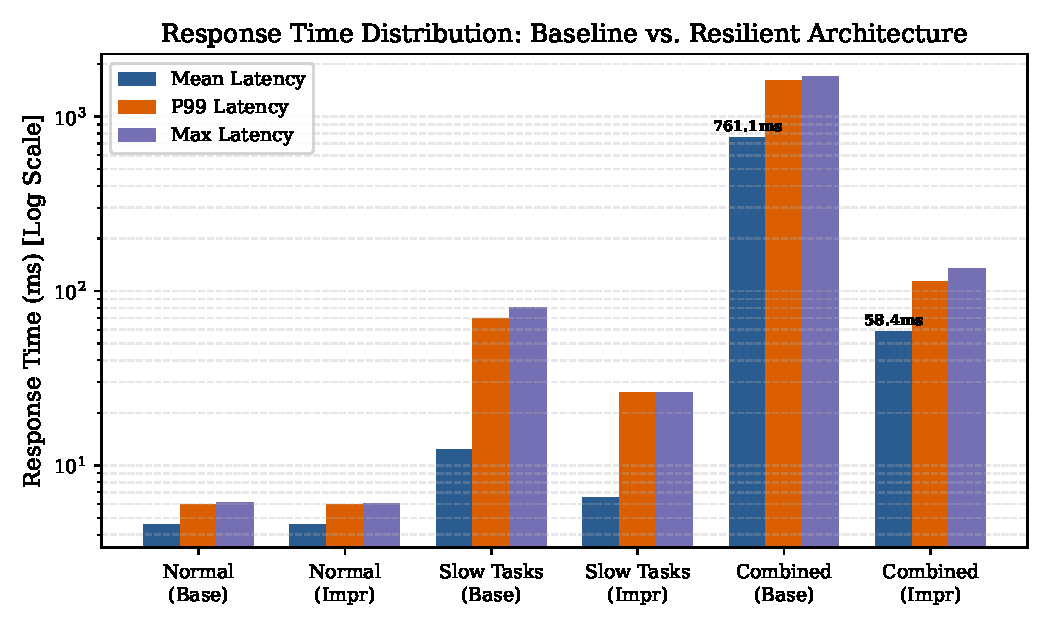
\includegraphics[width=\textwidth]{plot_latency_comparison.pdf}
        \caption{Latency Distribution (Mean, P99, Max on Log Scale)}
        \label{fig:latency}
    \end{subfigure}
    \hfill
    \begin{subfigure}[b]{0.48\textwidth}
        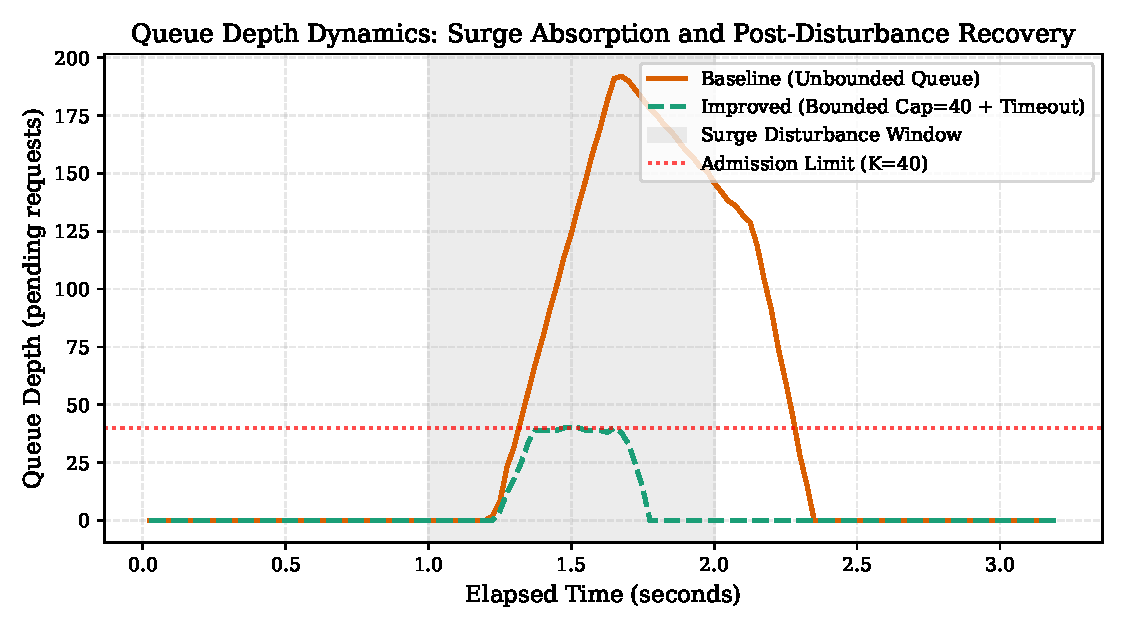
\includegraphics[width=\textwidth]{plot_queue_recovery.pdf}
        \caption{Queue Depth Profile and Surge Recovery}
        \label{fig:recovery}
    \end{subfigure}
    
    \vspace{0.3cm}
    
    \begin{subfigure}[b]{0.48\textwidth}
        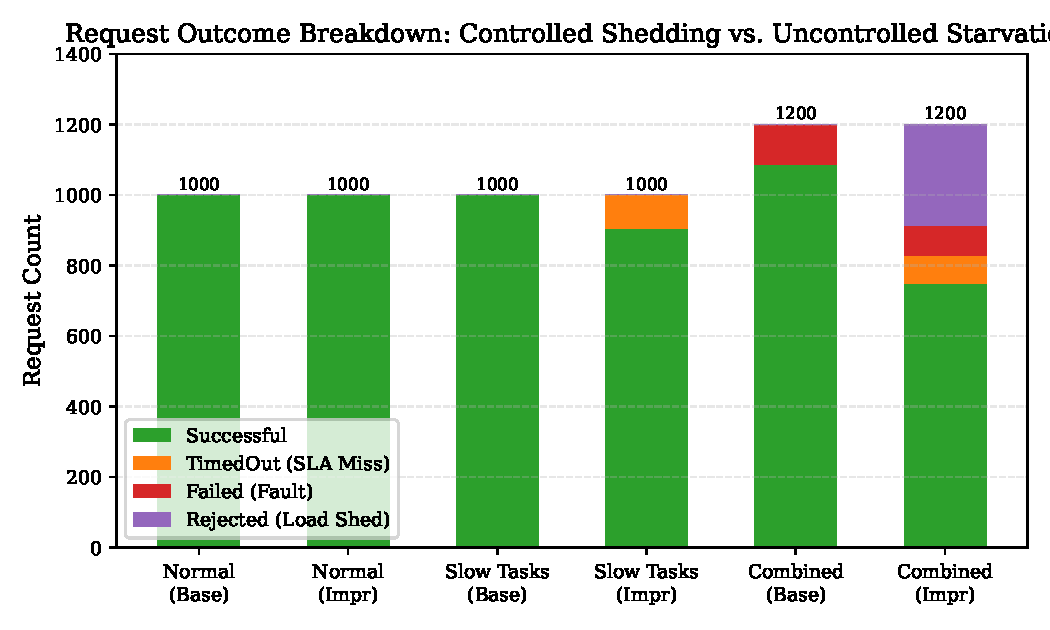
\includegraphics[width=\textwidth]{plot_outcomes_breakdown.pdf}
        \caption{Outcome Breakdown Under Adverse Stress}
        \label{fig:outcomes}
    \end{subfigure}
    \hfill
    \begin{subfigure}[b]{0.48\textwidth}
        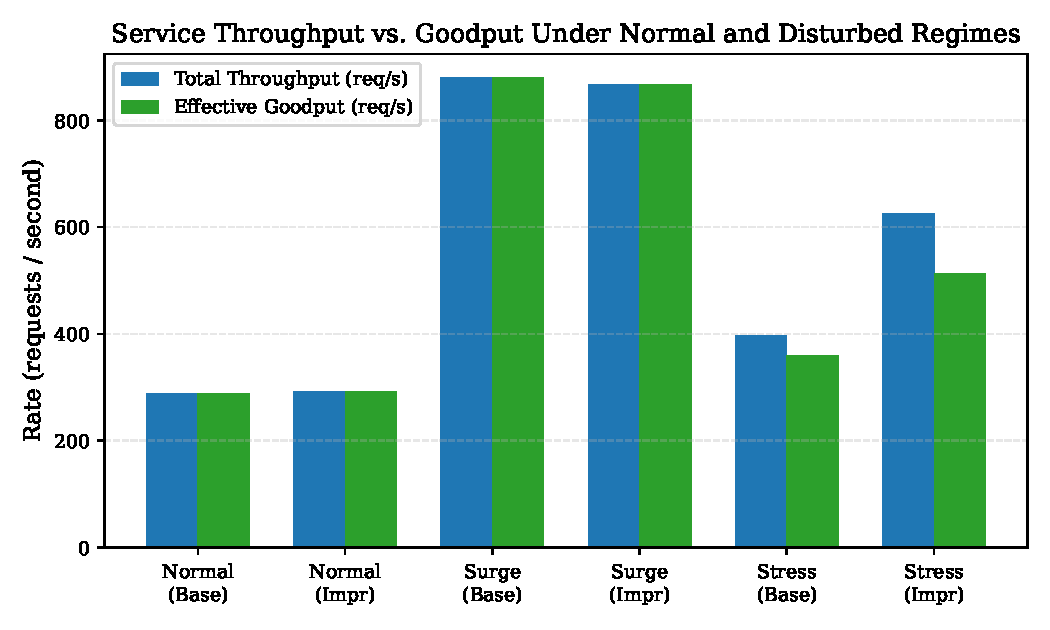
\includegraphics[width=\textwidth]{plot_throughput_goodput.pdf}
        \caption{Throughput vs. Goodput Across Regimes}
        \label{fig:throughput}
    \end{subfigure}
    \caption{Empirical Comparison: Baseline vs. Resilient Concurrent Service.}
    \label{fig:performance_plots}
\end{figure}

\subsection*{3. Analysis of Core Evaluation Questions}
\begin{enumerate}[label=\textbf{\arabic*.}, leftmargin=1.5em, itemsep=0.3em]
    \item \textbf{Which resilience mechanism produced the most significant improvement?}\\
    \textit{Context Timeout Cancellation.} While the bounded queue capped memory, context cancellation prevented worker starvation. Terminating the 8\% slow tasks at 25\,ms restored worker availability, raising throughput from 397.3 to 625.6\,req/s and preventing short tasks from queueing.
    \item \textbf{Did any improvement come at the cost of another desirable property?}\\
    Yes. Stability and low latency came at the expense of request rejection. Under combined stress, 288 requests were rejected ($24.0\%$) and 80 timed out ($6.7\%$). The baseline completed 1,086 requests ($90.5\%$), but with unacceptable 1.7-second delays.
    \item \textbf{Did the modified service reject requests that the baseline accepted?}\\
    Yes. The modified service rejected 288 requests that the baseline queued.
    \item \textbf{Did rejecting requests improve the experience of accepted requests?}\\
    Yes. For the 912 accepted requests, mean response time dropped from 761.13\,ms to 58.37\,ms (a 13-fold reduction), and max latency fell from 1,698\,ms to 134.87\,ms.
    \item \textbf{Did the service recover after the disturbance ended?}\\
    Yes. Figure~\ref{fig:recovery} shows that once the surge subsided, the improved queue drained within 50\,ms. In the baseline, a backlog of 196 requests took $>1.2$ seconds to drain, penalizing normal arrivals long after the surge ended.
    \item \textbf{General Resilience vs. Tested Conditions:}\\
    The design is structurally resilient against overload and slow dependencies because it enforces Little's Law bounds ($W_q \le K/\mu$) and prevents worker monopolization. However, the specific parameters ($K=50$, $\tau=25\,\text{ms}$) must be calibrated for target production workloads.
\end{enumerate}

\subsection*{4. Engineering Recommendation for University Deployment}
We recommend the following production architecture for the student request service:
\begin{enumerate}[leftmargin=1.4em, itemsep=0.15em]
    \item \textbf{Bounded Intake with Fast 503 Rejection:} Set intake capacity to $K \approx 2 \times W \times (\text{SLA} / \bar{S})$. When full, return HTTP 503 with a \texttt{Retry-After} header rather than allowing queue growth.
    \item \textbf{Tiered SLA Timeouts by Request Type:} Assign deadlines by service complexity: 50\,ms for certificate lookups; 250\,ms for administrative approvals.
    \item \textbf{Worker Pool Autoscaling with Hard Ceilings:} Base worker count on nominal load, with horizontal scaling triggered when average queue depth exceeds 70\% capacity for $>5$\,s, up to hardware core limits.
    \item \textbf{Continuous Queue Telemetry:} Track $\frac{dL}{dt}$, goodput, and rejection ratios to alert operators before worker exhaustion occurs.
\end{enumerate}


% --------------------------------------------------------------------------------------------
% REFLECTION AND DISCUSSION
% --------------------------------------------------------------------------------------------
\newpage
{\centering\fontsize{14}{17}\selectfont\textbf{Reflection and Group Discussion}\par}
\vspace{0.6em}

\begin{enumerate}[label=\textbf{Question \arabic*:}, leftmargin=1.5em, itemsep=0.45em]
    \item \textbf{Can a service be functionally correct but operationally unusable?}\\
    Yes. In the baseline stress test, the service was functionally correct: zero panics occurred, state was preserved, and all 1,200 requests were processed. However, response times reached 1.7 seconds. In production, client HTTP connections time out after 500\,ms; the server wastes work completing requests for clients that have already disconnected.

    \item \textbf{Why might adding more workers fail to solve an overload problem?}\\
    Adding workers fails when: (a) Arrival rate persistently exceeds physical capacity ($\lambda > \mu_{\max}$), where adding threads simply increases memory consumption and scheduler overhead; or (b) Downstream bottlenecks exist (e.g., database lock contention or disk saturation), where additional workers increase thread contention and degrade throughput further.

    \item \textbf{Is rejecting some requests necessarily a failure of the service, or can it be a deliberate resilience strategy?}\\
    Rejecting requests under overload is an intentional resilience strategy called \textit{load shedding}. A service has finite processing capacity. When load exceeds capacity, the system must either: (1) Accept all work and fail all users via latency collapse; or (2) Accept a sustainable volume within SLA and reject the rest. Rejection protects service goodput for accepted callers.

    \item \textbf{Under what circumstances can retry mechanisms worsen an existing problem?}\\
    Retries worsen issues during systemic resource exhaustion. When an overloaded service slows down, clients time out and issue retries. This amplifies incoming request volume ($\lambda_{eff} = \lambda \cdot (1 + r)$), increasing queue depth and causing further timeouts in a positive feedback loop (retry storm).

    \item \textbf{What is the difference between recovery of an individual component and resilience of the complete service?}\\
    Component recovery is local: restarting a crashed worker or reconnecting a database socket. Service resilience is architectural: the end-to-end service continues serving accepted traffic within SLAs and shedding excess load even while individual components are slow or failing.

    \item \textbf{How does this practical change your understanding of concurrency, performance, and dependability?}\\
    Concurrency is often treated as a tool for performance acceleration. This experiment showed that unconstrained concurrency (unbounded queues and unmonitored goroutines) causes severe latency collapse under load. Dependable concurrency requires control boundaries: bounded buffers, explicit admission control, and cooperative context cancellation.
\end{enumerate}

\vspace{0.8em}
\noindent\textbf{Statement of Individual Group Contributions:}
\begin{itemize}[itemsep=0.15em]
    \item \textbf{Gaurav Acharya [MT26MCS024]:} Formulated Part A claims classifications and queueing derivations; implemented the baseline Go concurrency pipeline, channel dispatcher, and thread-safe result collector; authored the test suite (\texttt{main\_test.go}) and race-detector verification; drafted the pre-coding response for Part D; implemented context timeout cancellation in Part E.
    \item \textbf{Sandeep [MT26MCS032]:} Designed and implemented bounded queue admission control and fast rejection in Part E; developed the Python plotting suite (\texttt{generate\_plots.py}) producing all comparative figures; ran benchmarks across all 11 configurations; drafted the comparative analysis, production recommendations, and reflection responses in Part F.
\end{itemize}

\end{document}
